\documentclass[12pt]{article}
\usepackage{amssymb,graphicx}
\usepackage{subfigure}
\usepackage[hyphens,obeyspaces,spaces]{url}
\usepackage{amsmath}
\usepackage{amsfonts}
\usepackage{amssymb}
\usepackage[T1]{fontenc}
\usepackage{carolmin}
\usepackage{t1enc}
\usepackage{color}
%\usepackagqe{times}
\usepackage{textcomp}
%\usepackage{natbib}

\def\eop{\hfill{$\vcenter{\hrule height1pt \hbox{\vrule width1pt
height5pt \kern5pt \vrule width1pt} \hrule height1pt}$}}

\newcommand{\bydef}{\mbox{$\:\stackrel{\triangle}{=}\:$}}
\newcommand{\insmat}[1]{\mathop{\rm {#1}}}  % for mathmode (with underlines)
\newcommand{\half}{{\textstyle\frac{1}{2}}}
\newcommand{\norm}[1]{\|#1\|}
\newcommand{\argmin}{\insmat{arg\,min}}
\newcommand{\argmax}{\insmat{arg\,max}}
\newcommand{\dist}{\insmat{dist\,}}
\newcommand{\aff}{\insmat{aff\,}}
\newcommand{\cl}{\insmat{cl\,}}
\newcommand{\conv}{\insmat{conv\,}}
\newcommand{\Qh}{\widehat{{\Omega}}}
\newcommand{\gammapQ}{\gamma_{p {\Omega}}}
\newcommand{\Pmu}{\mathbb{P}_\mu}
%\linespread{3.0} %For JOTA format


\begin{document}
%\noindent
%\begin{center}
%\large \textbf{Suboptimality of minmax MPC}
%\vspace{0.5cm}
%\noindent
%\vspace{0.5cm}
%\end{center}

\noindent
\begin{center}
 \textbf{MPC Path 	Planner}
\vspace{0.5cm}
\noindent
\vspace{0.5cm}
\end{center}

At current time, solve following optimization problem. $N$ is horizon length, $M$ is the number of detected obstacles. The pair $z_k:=(x_k,y_k)$ is a position of vehicle at time $k$.$\tau^i_k$ is the position of $i^{th}$ obstacle (vehicles) at time $k$. $T$ is a goal position, $f_z$ and $f^i_{\tau}$ are dynamics for ego vehicle and $i^{th}$ obstacle. There are two kinds of obstacles. Static obstacle and dynamics obstacle (other vehicle).

\begin{equation}
\begin{split}
&\min_{u\in U}\sum_{k=1}^ND^2_k(z_k)+\sum_{i=1}^M\sum_{k=1}^NP_k^i(z_k,\tau^i_k)\\
s.t.&~~z_{k+1}=f_z(z_k,u_k),\\
&~~\tau_{k+1}=f_\tau(\tau_k,u_k),\\
&~~\textit{Comfort constraint},
\end{split}
\end{equation}
where
\begin{equation}
\label{penalty}
P_k^i(z_k,\tau^i_k) := w\frac{\exp(-\alpha(\|z_k-\tau_k^i\|^2-s^2))}{1+\exp(-\alpha(\|z_k-\tau_k^i\|^2-s^2))}
\end{equation}
\begin{equation}
D_k(z_k)=\|z_k - T \|
\end{equation}


$P_k^i$ applies large penalty to the position of the $i^{th}$ obstacle that is located at $\tau^i$ at time $k$. 

Fig.1 shows the effect of two tuning parameters $s$ and $\alpha$.
horizontal axis is $x$, vertical axis is $z$ for both subfigures.
\begin{figure}[h!]
\begin{centering}
\subfigure[Parametrized by $s$]{
	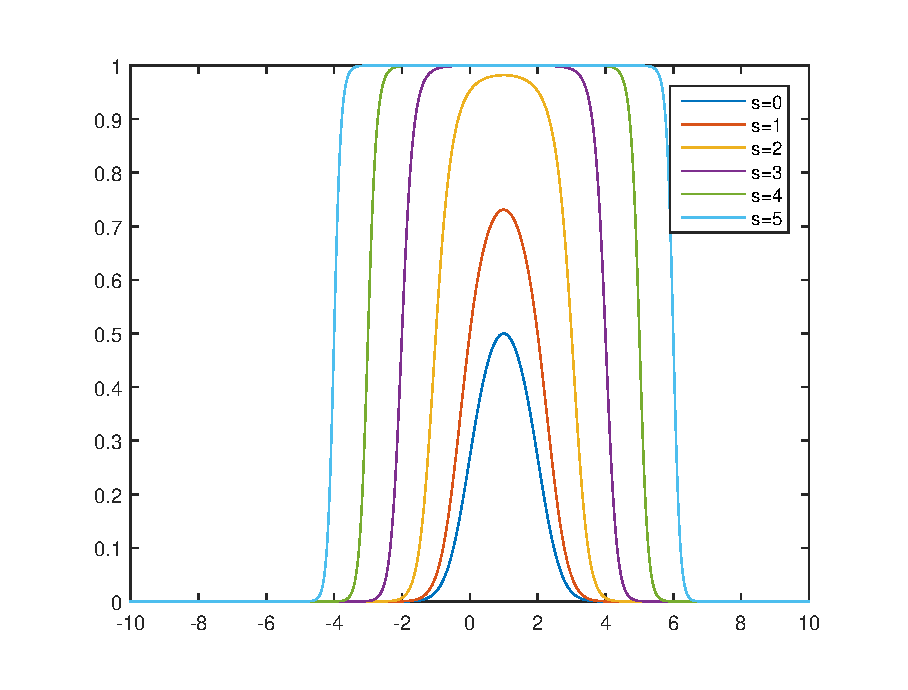
\includegraphics[width=10cm]{./Figures/bell1.eps}
	}
\subfigure[Parametrized by $\alpha$]
	{
	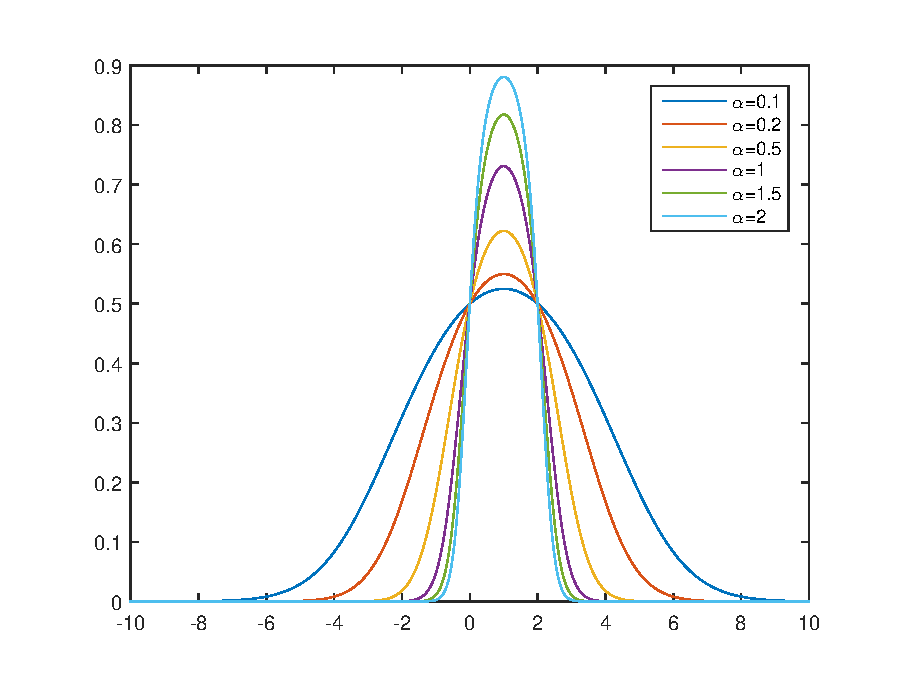
\includegraphics[width=10cm]{./Figures/bell2.eps}
	}
\par\end{centering}
\caption{Penalty term parameterized by $s$ and $\alpha$ }
\end{figure}
As shown in Fig.1(a), the parameter $s$ determines the range of penalty effect and the parameter $\alpha$ determines growing rate of the penalty. In the future, both parameters could be a function of speed of vehicle.

Note that Eq.(2) realizes cut-in and yield(let others to cut in) plan. 

\subsection*{Lane Change}
Choosing goal position $T$ is a design parameter. If $T$ is located in the center line of any lane, vehicle path converge to the corresponding lane.

\subsection*{Goal Position}
Goal should be set based on traffic information such as high way exit location, road merge and so on. 
\end{document}